\documentclass[letterpaper, 12pt]{article}
\usepackage{geometry}
\geometry{
    letterpaper,
    left=20mm,
    top=20mm,
    bottom=20mm
}
\usepackage{tocloft}
\usepackage{graphicx}
\usepackage{authblk}
\usepackage{amssymb}
\usepackage{lipsum}
\usepackage{float}
\usepackage{times}
\usepackage{amsmath}
\usepackage[format=plain,
            labelfont={bf,it},
            textfont=it]{caption}
\captionsetup{justification=raggedright,singlelinecheck=false}
\usepackage{ragged2e}
\usepackage{longtable}
\usepackage{comment}
\usepackage{setspace}
\usepackage{fancyhdr}
\usepackage{titlesec}
\usepackage[hyperindex,breaklinks]{hyperref}
\hypersetup{
    colorlinks=true,
    linkcolor=blue,
    filecolor=magenta,      
    urlcolor=blue
}
\usepackage[T1]{fontenc}
\usepackage{helvet}
\renewcommand{\familydefault}{\sfdefault}
\pagenumbering{gobble}
\usepackage[skip=10pt plus1pt, indent=40pt]{parskip}
\usepackage{orcidlink}
\usepackage{standalone}

\titlespacing*{\section}
{0pt}{1.5ex plus 1ex minus .2ex}{1.3ex plus .2ex}

\renewcommand\Authfont{\fontsize{12}{14.4}\selectfont}
\renewcommand\Affilfont{\fontsize{9}{10.8}\itshape}

\newcommand{\cosigpart}[1]{
  \addcontentsline{toc}{part}{#1}
}
\newcommand{\cosigsection}[1]{
  \section*{#1}
  \phantomsection % avoid warnings from hyperref about the anchor of a bookmark and its parent's
  \addcontentsline{toc}{section}{#1}
}
\begin{document}
\flushleft
\includegraphics[width=0.5\textwidth]{img/home/241017_final_logo_mockup.png}

\cosigsection{Granularity-related inconsistency of means (GRIM)}
\textit{Last updated: 13 June 2025}

% Reese: Let's restrict this guide to just be about GRIM--GRIMMER requires a bit more explanation, as do SPRITE/CORVIDS/DEBIT/etc. Each can occupy their own guide!

Imagine that we ask two participants their age in years then report their mean age rounded to one decimal place. No matter these two participants' ages, their mean age must end in either .0 or .5, because the average of any two integers must either be a whole number (if both ages are odd or both ages are even) or an integer plus .5 (if one is even and one is odd). It would be impossible for the participants' mean age to end in, say, .2. Similarly, if we ask five participants their age, their mean age must end in .0, .2, .4, .6 or .8. It would be impossible for five participants' mean age to end in, say, .3. When the underlying data has known granularity (e.g., only integers) and the total number of observations is known (e.g., sample size or N), only some means are mathematically possible. Similarly, if we ask five participants if they are currently students or not and then report the percentage of participants that are students, this percentage could only ever be 0\%, 20\%, 40\%, 60\%, 80\% or 100\%. It would be impossible for, say, 45\% of our five participants to be students.

These principles underlie testing for granularity-related inconsistency of means (GRIM or GRIM testing, see \href{https://jamesheathers.medium.com/the-grim-test-a-method-for-evaluating-published-research-9a4e5f05e870}{Heathers, 2016a}, \href{https://jamesheathers.medium.com/the-grim-test-further-points-follow-ups-and-future-directions-afd55ff67bb0#.vmgjvdvkf}{Heathers, 2016b}, and \href{https://doi.org/10.1177/1948550616673876}{Brown and Heathers, 2017}). Notably, GRIM testing only requires access to the summary statistics that are commonly reported in articles, not necessarily to the raw data underlying these summary statistics (however, it is always preferable to have access to the raw data to understand if/how any data has been misreported).

%Many quantitative research articles report the total number of observations (sample size), means, percentages, and/or standard deviations. Under certain conditions related to the granularity of the raw data, only some means, percentages, and standard deviations are possible for a given sample size. Under certain conditions, it is therefore possible to check whether reported means, percentages, or standard deviations are mathematically possible given reported sample sizes. 

%These granularity-based methods for assessing consistency are referred to as GRIM (Granularity Related Inconsistency of Means: \href{https://jamesheathers.medium.com/the-grim-test-a-method-for-evaluating-published-research-9a4e5f05e870}{Heathers (2016a)}, \href{https://jamesheathers.medium.com/the-grim-test-further-points-follow-ups-and-future-directions-afd55ff67bb0#.vmgjvdvkf}{Heathers (2016b)}, \href{https://doi.org/10.1177/1948550616673876}{Brown \& Heathers (2017)}) and GRIMMER (an extension for standard deviations, see \href{https://aurelienallard.netlify.app/post/anaytic-grimmer-possibility-standard-deviations/}{Allard (2018)}; \href{https://peerj.com/preprints/2400/}{Anaya (2016)}; \href{https://jamesheathers.curve.space}{Heathers, (2025a)}). Checking for such inconsistencies between reported sample size and summary statistics can be an efficient and useful way of checking the trustworthiness of research \href{https://doi.org/10.1177/1948550616673876}{Brown, N., \& Heathers, J. (2017). 

%GRIM and GRIMMER, which this guide collectively refers to as GRIM/MER, are useful because they do not require access to the raw data, only to numbers that are commonly reported in articles. This can be useful in the direct sense that GRIM/MER can form part of a trustworthiness assessment without needing access to the data, which is often not shared. GRIM/MER can also be useful in an indirect sense, as observing several GRIM/MER inconsistencies can provide a rationale to approach authors, or indeed journal editors or publishers' research integrity teams, with a request for the underlying data to further assess trustworthiness. 

Common use cases of GRIM testing include, but are not limited to:

\begin{itemize}
    \setlength\itemsep{-0.5em}
    \item Demographic summary statistics, often reported in an article's text or in a table in medical and epidemiological articles;
    \item \href{https://en.wikipedia.org/wiki/Factorial_experiment}{Factorial experiments} reporting number of observations and mean of observations;
    \item Mean values of questionnaire answers collected on a \href{https://en.wikipedia.org/wiki/Likert_scale}{Likert scale} (e.g., ``How happy are you?'' on a scale from 1 to 7 with 1 being least happy to 7 being most happy);
    \item Meta-analysis forest plots reporting number of observations and mean.
\end{itemize}
\href{https://doi.org/10.17605/OSF.IO/M82S6}{Heathers (2024)} describes additional uses of GRIM (e.g., to recover cell counts used to calculate \href{https://en.wikipedia.org/wiki/Chi-squared_test}{chi-squared tests}).

% GRIMMER, the extension of GRIM to standard deviations and variances, follows a generalization of the logic of GRIM with slightly more complex math (see \href{https://aurelienallard.netlify.app/post/anaytic-grimmer-possibility-standard-deviations/}{Allard (2018)}; \href{https://jamesheathers.curve.space}{Heathers (2025a)}). For simplicity, the below explanations will focus on GRIM and reported means, but the same logic applies to proportions and percentages (via GRIM) as well as standard deviations and variances (via GRIMMER).

GRIM testing involves determining which mean values reported in an article are mathematically possible. The precise values that are determined to be mathematically possible (i.e., the values which ``pass'' GRIM testing or are ``GRIM-consistent'') depend on six factors, discussed below.

\subsubsection*{Precision of the reported estimates}

The utility of GRIM is highly dependent on the precision of reporting (i.e., the number of decimal places to which means or other estimates are reported). The more decimal places are reported, the lower the proportion of mathematically possible values. For instance, if 20 people are asked their age and the mean age is reported with a precision of one decimal place, it is possible for their mean age can end in any digit, .0 through .9. However, if their mean age is reported to two decimal places, certain ending digits would not be possible (e.g., 21.07 would not be possible because there is no integer sum of ages that, when divided by 20, would result in a number with two decimal places ending in 7. All possible means with two decimal places would end in 5 or 0).

\subsubsection*{Number of observations (sample size or N)}

The utility of GRIM testing is highly dependent on the total number of observations (i.e., sample size or N). The smaller the sample size, the lower the proportion of mathematically possible values, and therefore the less probable it is that misreported or fabricated means will pass GRIM testing. The specific calculation of sufficient granularity due to sample size and number of items is discussed further below, but a basic rule of thumb (useful for summary statistics reported to 2 decimal places) is that GRIM testing is only useful when the sample size is less than 100. 

\subsubsection*{Rounding method used}

Rounding matters for GRIM. Articles report estimates to a given precision (e.g., two decimal places), and may employ different rounding methods when calculating these values. For example, the mean age in years of any three participants reported to two decimal places must end in .00, .33, or .67. But what if the authors simply truncated the values, so that .666666 became .66 rather than .67? Additional values may pass GRIM testing based on multiple possible rounding methods. Many implementations of GRIM allow you to specify either a specific rounding method, if it is known, or to allow for both round-up and round-down methods. 

Variations in rounding methods are fairly common. In daily life, most use the round-half-up method where numbers that are exactly between two integers are rounded up to the nearest integer (e.g., 1.5 is rounded to 2, 2.5 is rounded to 3 and so on). This is not the default method used in many programming languages, including R and Python 3, which use ``banker's rounding'': values ending in 5 are rounded up or down based on the preceding digit being odd or even. For example:
\begin{verbatim}
round(1.5) # returns 2
round(2.5) # returns 2
round(3.5) # returns 4
round(4.5) # returns 4
round(5.5) # returns 6
round(6.5) # returns 6
\end{verbatim}
This form of rounding is the default in many programming languages because it minimizes the overall rounding error when individual elements of a computation are rounded.

\begin{comment}

Consider the following table reporting mock summary statistics for integer data (adapted from the \href{https://errors.shinyapps.io/scrutiny/}{scrutiny web app})

\begin{center}
\begin{tabular}{|p{3.0cm}|p{3.0cm}|p{3.0cm}|p{3.0cm}|}
\hline
    Group & Mean & Standard deviation & N\\ \hline\hline
    A & 7.22 & 5.30 & 38\\ \hline
    B & 4.74 & 6.55 & 31\\ \hline
    C & 5.23 & 2.55 & 35\\ \hline
    D & 2.57 & 2.57 & 30\\ \hline
    E & 6.77 & 2.18 & 33\\ \hline
    F & 2.68 & 2.59 & 34\\ \hline
    G & 7.01 & 6.68 & 35\\ \hline
    H & 7.38 & 3.65 & 32\\ \hline
    I & 3.14 & 5.32 & 33\\ \hline
    J & 6.89 & 4.18 & 37\\ \hline
    K & 5.00 & 2.18 & 31\\ \hline
    L & 0.24 & 6.43 & 34\\ \hline
\end{tabular}
\end{center}

\end{comment}

% Reese: PDF version of figure is smaller size but loads too many objects, slowing down PDF rendering. Need to plot as an image in order to use PDF here.
\begin{figure}[h!tbp]
    \centering
    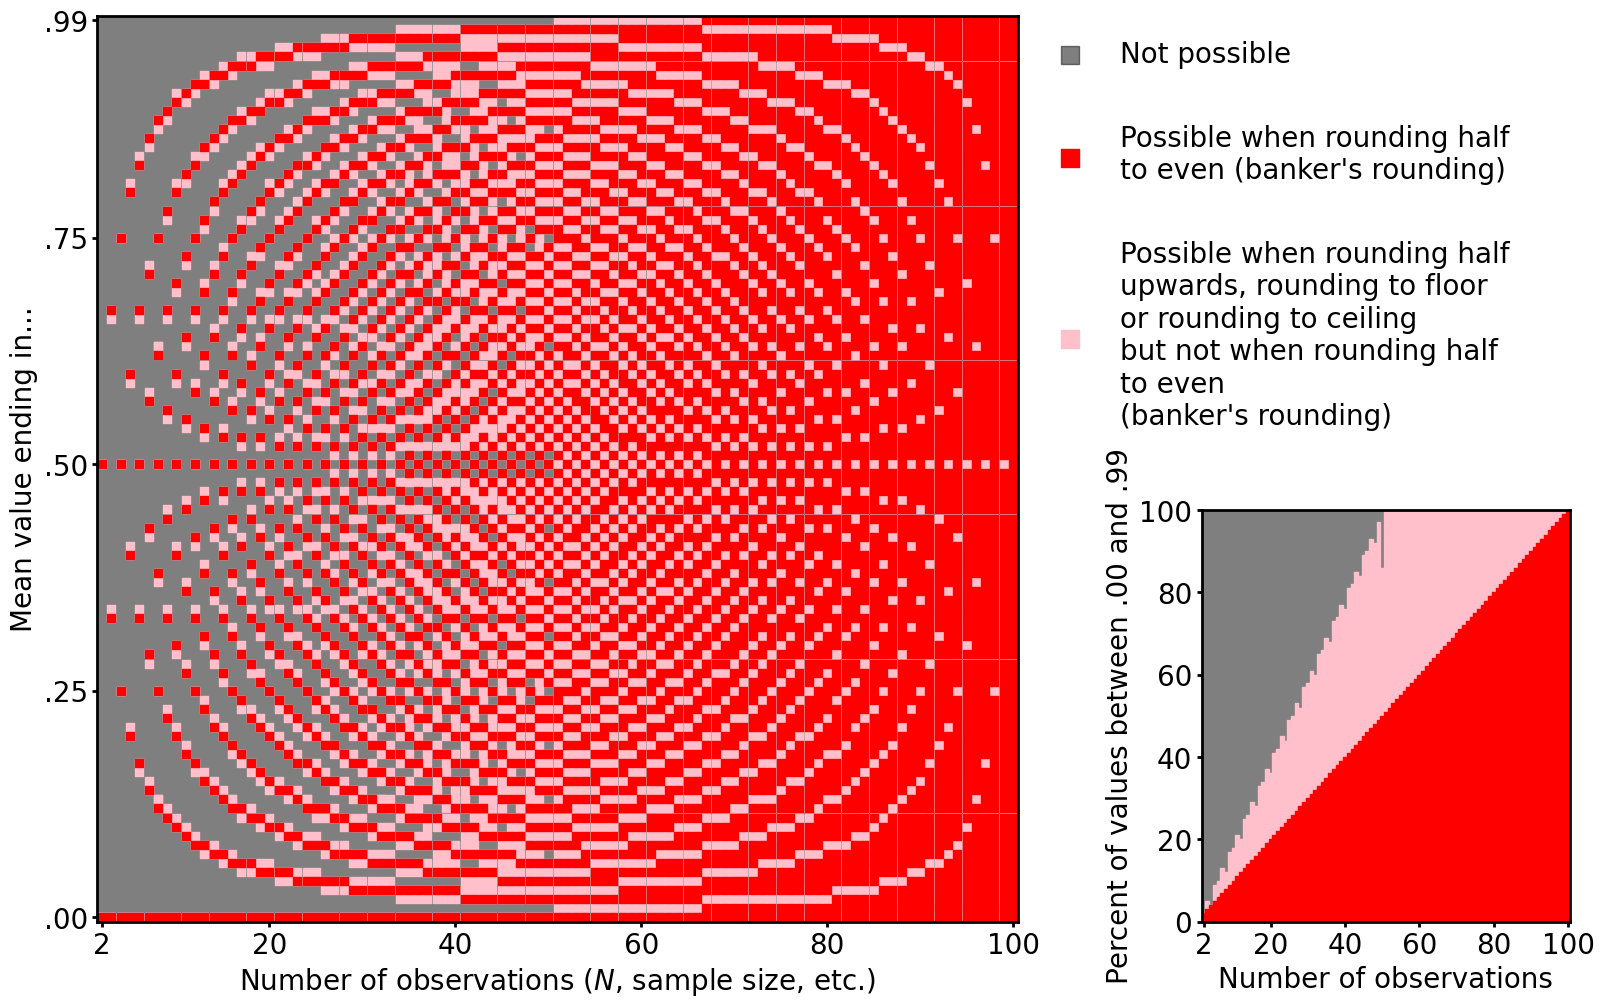
\includegraphics[width=\linewidth]{img/grim/250612_grim_possibilites_r2.png}
    \caption*{This figure shows which mean values are possible when dividing a sum of positive integer measures over a number of observations between 0 and 100 (N) and rounding to two decimal places. Gray squares indicate values that are not mathematically possible under any rounding procedure. Red squares indicate values that are mathematically possible when rounding numbers halfway between two numbers to the nearest even value (``banker's rounding'', the default method used in many programming languages). Pink squares indicate values that are mathematically possible only when using an atypical rounding procedure (like rounding down, rounding up, or rounding numbers halfway between two numbers upwards). The smaller plot shows the proportion of values between .00 and .99 that are mathematically possible under each rounding procedure. Notice that as N increases, more values will pass GRIM testing and for smaller N, a greater proportion of values are mathematically impossible.}
\end{figure}

\subsubsection*{Granularity of the measurement instrument}

GRIM testing requires that the measurement instrument produces granular data. For example, participants' ages in years should usually only be recorded as integers (whole numbers), such as 21, 28, or 39, but not as fractions such as 21.5. GRIM can be used on any measurement instrument with known or reasonably-assumed granularity. GRIM cannot be used on data with no granularity or arbitrary granularity. Truly continuous data with an arbitrary number of decimal places (e.g., height of participants) do not place any constraints on what sample means can be obtained. Most data recorded in behavioral studies do have some degree of granularity (e.g., \href{https://en.wikipedia.org/wiki/Likert_scale}{Likert scales}, reaction times in milliseconds, counts of events, etc.). Realistically, any measure has some amount of granularity equal to the precision of the reporting instrument (e.g., although weight is continuous, most scales will only report weight to one decimal place).

Common implementations of GRIM assume that the raw data are integers, such as with single Likert scales. GRIM testing may not be useful if the measurement instrument that generated the data has sufficiently fine granularity so as not to put any constraints on means. For example, with the \href{https://en.wikipedia.org/wiki/Visual_analogue_scale}{Visual Analogue Scale}, participants' responses are not necessarily integers but can take value from 0.00 to 10.00 with two decimal places, making any average of these scores reported with two or fewer decimal places GRIM-consistent.

When a single item measure on an integer scale is used (e.g., participant age, rating from 1 to 5 stars, single-item Likert scale response, etc.), all means will pass GRIM testing when $N \geq 10^{d \cdot i}$, where $N$ = number of observations, $d$ is the precision or number of digits the mean is reported to and $i$ is the number of items already averaged over. 

\subsubsection*{Number of items averaged over at the participant level}

Sometimes, measures are averages over multiple items. For example, a questionnaire might include five questions that are scored on a self-reported Likert scale, where the measure of interest is each participant's mean score on these five questions (i.e., there are five items averaged over at the partipant level). Assuming that the participant answered every question, each partipants' mean score on these five questions must end in .0, .2, .4, .6 or .8. This is factored into the calculation of values that pass GRIM testing by multiplying the number of items averaged at the participant level by the number of participants averaged over for the sample mean. For many software implementations of GRIM (detailed later in this guide), the parameter representing the number of items averaged over at the participant level is called \texttt{items}. If, instead of taking the mean at the participant level the sum of each question is taken (e.g., the seven-point (1-7) Likert-scale answers to all five questions are summed up into a composite score with range 5 to 35), \textit{items = 1}. Most singular measurement instruments (e.g., ``age in years'' or a single answer to a Likert-scale question) are single-item measures, so \texttt{items = 1}.

%Implicitly, a measurement instrument such as ``age in years'' is a single item measure, so \texttt{items = 1}. Equally, a common source of confusion for users of GRIM/MER is setting \texttt{items} to the number of items in a multi-item self-report scale. For example, setting \texttt{items = 21} for the Beck Depression Scale, which has 21 items. The important nuance here is that, regardless of the specific implementation of GRIM/MER, \texttt{items} refer not to the number of items in scale, but rather the number of items already averaged over at the participant level before then calculating the sample mean (or percent, standard deviation, etc.). So, if the scale was sum-scored, which is very common in psychology, no averaging occurred before the sample mean was calculated. The Beck Depression Inventory is usually sum-scored, so \texttt{items = 1}. In contrast, if mean scoring was used at the participant level, then the number of items is the averaged value. Note that mean scoring can also raise issues related to missingness that can throw off GRIM/MER (see section below). 

\subsubsection*{Poor documentation of methodology}

GRIM testing may be misled by unreported methodological steps undertaken by the researchers. For instance, imagine a study where participants were asked to circle their response from 1 to 5 on a pen-and-paper questionnaire, some participants put one circle around two adjacent numbers (e.g., 2 and 3) and the researchers elected to record this value as the midpoint (2.5) without reporting this methodological choice in the article. This methodological step reshapes what mean values are mathematically possible and complicates GRIM-testing. Similarly, an article may report that participants recorded their age as an integer, but the online form used to collect data allowed participants to enter their age to one decimal place (e.g., 21.5). 

Researchers are expected to report all relevant methodological choices in an article. If you find that certain values reported in an article fail GRIM testing, consider whether certain undocumented methodological choices could have produced these values. Similarly, consider whether authors may have misreported the number of participants (e.g., ``20 participants'' was accidentally misreported as ``21 participants'').

GRIM testing can also be complicated by missing data at the participant level. For example, if the measurement instrument was reported to be a five-item self-reported Likert scale that was mean-scored at the participant, we would expect each participant's mean score ends in .0, .2, .4, .6 or .8. This places constraints on what the sample mean scores can plausibly be (and \texttt{items} would be set to 5 when calculating GRIM, as five items were averaged over at the participant level before calculating the sample mean). However, if a participant had missing data, this would throw off the calculation of GRIM for the sample mean. For example, if a participant only provided responses to four of the five Likert items, their mean score would have to end in .00, .25, .50 or .75. When an unknown number of participants has missing data because this was not reported in the article, this could make it impossible to correctly determine which sample means are GRIM-consistent.

\begin{comment}
    
\section*{Usage}

\subsection*{Reported results needed to use GRIM/MER}

GRIM/MER are useful when sample sizes are relatively small (often <100) and the measure that generated the data is one that records integer values (e.g., Likert scale data or categorical responses). This is often the case in psychological data.

GRIM: 
  \begin{itemize}
      \item The sample size (N) and a mean, proportion, or percentage from the same data set.
      \item The granularity of the measure used to collect the data, e.g., whether only integer values are possible in the raw data, and how many items were averaged over.
  \end{itemize}

GRIMMER:
  \begin{itemize}
      \item The sample size (N) and a standard deviation or variance from the same data set.
      \item The granularity of the measure used to collect the data: e.g., whether only integer values are possible in the raw data, and how many items were averaged over.
  \end{itemize}

\subsection*{Limitations to GRIM testing}

\subsubsection*{Fine granularity}

Common implementations of GRIM assume that the raw data are integers, such as with single Likert scales. GRIM testing may not be useful if the measurement instrument that generated the data has sufficiently fine granularity so as not to put any constraints on means. For example, with the \href{https://en.wikipedia.org/wiki/Visual_analogue_scale}{Visual Analogue Scale}, participants' responses are not necessarily integers but can take value from 0.00 to 10.00 with two decimal places, making any average of these scores reported with two or fewer decimal places GRIM-consistent.

When a single item measure on an integer scale is used (e.g., participant age, rating from 1 to 5 stars, single-item Likert scale response, etc.), all means will pass GRIM testing when $N \geq 10^{d \cdot i}$, where $N$ = number of observations, $d$ is the precision or number of digits the mean is reported to and $i$ is the number of items already averaged over. 

%Of course, multi-item self-report scales are also common, and this can have implications for the utility of GRIM/MER. Beyond a certain point, all reported means will pass GRIM, even if the means were completely fabricated and no data set ever existed. To take the simple common situation where means are reported with two decimal places and the measure is a single item measure that produces integers (e.g., ``what is your age in years?''), all means will pass GRIM when $N \geq 10^{d \cdot i}$,

%For example, for a single item measure such as ``what is your age?'', $i$ = 1. If a multi-item self-report scale was used, $i$ depends on whether the scale was sum-scored or mean-scored. If mean-scored this ``uses up'' some of the constraint on granularity available in the sample mean, because data has been averaged twice, once at the participant level and once at the sample level. For a ten-item scale that was mean-scored, $i$ = 10. However, if sum-scoring was used, no granularity has been 'used up' because no averaging has taken place before the sample mean was calculated, so $i$ = 1. 

%Similarly, according to Nick Brown, GRIMMER will pass most values when the number of observations is greater than about 30 (assuming a precision of two decimal places and a value of $i$ of 1). This rule of thumb has yet to be empirically simulated. 

\end{comment}

\begin{comment}

\section*{Interpretation and misinterpretation}

\subsection*{False positives due to mistakes on your behalf}

The bar for critique is typically higher than the bar for publishing the original research itself. As with any trustworthiness assessment or critique, start by making sure you have not made a mistake yourself. For example, did you correctly extract the sample size, means, or other estimates, did you correctly infer the number of items already averaged over (see above for a common misconception about multi-item self-report scales), etc. 

\subsection*{False or pseudo positives due to unreported features of the method}

Sometimes, granularity can be different than that implied by the reported method, such as a lack of constraints on responses in the measurement instrument or unreported data cleaning steps. For example, the article might report that participants were asked their age, but the online survey may have allowed participants to enter years with decimal places (e.g., 23.5). If one or more participants did so, this could produce failed GRIM/MER tests. This is not technically a false positive: the failed GRIM/MER test could correctly determine that the mean cannot be produced under the methods reported in the article and the assumptions made by the researcher running the GRIM/MER test, which warrants further examination, even if the reason for this failure turns out to be relatively innocuous.

To hedge against such false positives, users of GRIM/MER should also check whether other values for the sample size produce summary statistics that pass GRIM/MER. Sometimes, one can work out that while the reported N = 20 makes the reported mean fail GRIM, simply using N = 19 makes it pass. A credible explanation can be the failure to disclose an exclusion in the article. Equally, failed GRIM/MER tests that have no nearby numbers that could pass may provide additional reason to lower our trust in the reported results. This process of attempting to backwards engineer what was likely to have actually happened in study is common to many forensic meta-science methods. Some implementations of GRIM/MER allow you to easily create GRIM/MER plots that also show whether nearby values of mean or sample size produce passing or failing values. 
\end{comment}

\subsection*{Limitations of GRIM testing}

\subsubsection*{GRIM testing does not account for range violations}

GRIM only assesses granularity but not other constraints such as range. For instance, if the reported mean of 10 participants' responses on a 1 to 7 Likert scale was 8.5, this would pass GRIM, but this mean is impossible based on the scale's range as the mean cannot be greater than the maximum allowable response value. For assessing range violations, consider using TIDES: \href{https://github.com/ianhussey/tides}{Hussey et al. (2024)}. 

\subsubsection*{Completely fabricated results may still pass GRIM}

It is important to recognize that GRIM only tells you whether a reported mean, proportion or percentage could have been calculated from a given vector of observations. It tells you nothing about the provenance or legitimacy of the underlying data. In the extreme case of fabrication of an entire data set, the mean of those fabricated values can trivially pass GRIM. Passing GRIM testing does not tell that the data is not fabricated. Failing it does not tell you it is fabricated either, merely that the description of the data generating process cannot produce the summary statistics that were reported. There are many reasons why these tests might fail, ranging from typos and the use of the wrong sample size (e.g., before versus after exclusions) to fabrication of the reported results without using any real underlying dataset. 

\begin{comment}
\subsection*{Probability of randomly generated means passing GRIM}

To meaningfully interpret the results of one or more GRIM tests, it is important to consider the probability that a randomly generated mean value will pass GRIM for a given number of observations N. As discussed above, the smaller the sample size, the fewer values of the mean can pass GRIM. The corollary of this is that as the sample size grows, more and more values of the mean would pass GRIM, even if those means were completely fabricated and no underlying data exists. This can be illustrated with a GRIM plot, as generated using {scrutiny} R package. In the plot in Figure %\ref{grimfig:figure-1}, the Y-axis shows each possible value of the mean (in this case actually a proportion) and is calculated based on the precision of the reported value (e.g., all values from the minimum to the maximum value of the scale, in increments of 0.01). The X-axis shows different sample sizes. White spaces in the plot indicate reported means that would pass GRIM, whereas gray squares indicate reported means that fail GRIM. Although they are not key to the point being made here, blue and red squares represent the actual reported values of mean and sample size that were provided to the test: with blue squares represent passes wheres red squares represent failures. The key insight to be taken from this plot is the relative transition from mostly gray squares on the left-hand side of the plot to very few gray squares on the right-hand side of the plot. That is, when sample sizes are low, few randomly generated reported means will pass GRIM; whereas when sample sizes are high, many will pass GRIM despite being randomly generated (fictitious) values. 
\begin{figure}[h!]
    \centering
    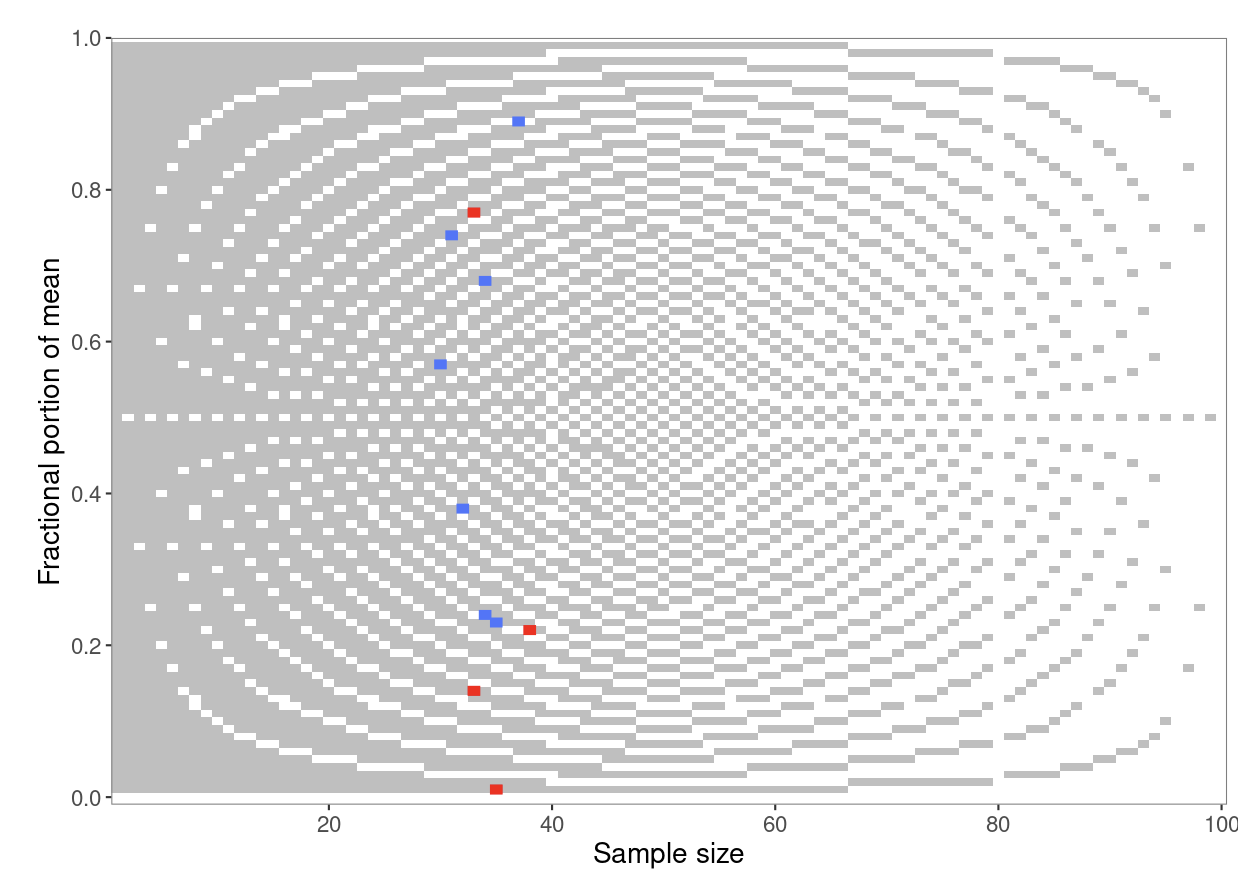
\includegraphics[width=0.5\linewidth]{img/grim/grim plot.png}
    \caption{Means that pass or do not pass GRIM based on sample size}
    %\label{grimfig:figure-1}
\end{figure}
This insight is useful and important when interpreting the result of one or more GRIM test, especially when interpreting multiple values. It is important to consider not merely the proportion of values in an article that pass GRIM, but the difference between the baseline probability of passing GRIM at that sample size. For example, imagine that you extract 10 means from an article, all of which are based on a sample size of N = 70, and all of which are reported to two decimal places and were obtained using a single-item measurement instrument. If 7 out of 10 items pass GRIM, what should you infer about the means? The majority of the values passed GRIM, so a user may interpret this as evidence of the means' legitimacy. However, for this sample size and precision and granularity, 70\% of randomly generated means would pass GRIM. As such, the observed results are precisely in line with what would be observed with a set of generated by something other than a legitimate data generating process as described in the article, and would therefore be sufficient to mark the means as implausible within the context of a trustworthiness assessment. Additional information should then be sought from the authors regarding whether some unreported feature of the method could explain this pattern of results, as well as the raw data for further inspection. 

\subsection*{False negatives due to completely fabricated data}

It is important to recognize that GRIM/MER only tells you whether a reported mean (or other summary stat) could have been calculated from a given vector of observations. It tells you nothing about the provenance or legitimacy of the underlying data. In the extreme case of fabrication of an entire data set, the mean of those fabricated values can trivially pass GRIM. So, passing GRIM does not tell that the data is not fabricated, and failing it does not tell you it is fabricated. It merely tells you that description of the data generating process cannot produce the summary statistics that were reported. There are many reasons why these tests might fail, ranging from mere typos or the use of the wrong sample size (e.g., before vs. after exclusions) to fabrication of the reported results without any underlying dataset. 

\end{comment}

\subsection*{Extensions of GRIM}

Extensions of GRIM testing include:

\begin{itemize}
    \setlength\itemsep{-0.5em}
    \item \textbf{GRIMMER, granularity-related inconsistency of means mapped to error repeats}, a method for testing whether reported values for variability (e.g., standard deviation and standard error) are mathematically possible. See \href{https://doi.org/10.7287/peerj.preprints.2400v1}{Anaya (2016)} and \href{https://aurelienallard.netlify.app/post/anaytic-grimmer-possibility-standard-deviations/}{Allard (2018)}.
    \item \textbf{DEBIT, \textit{DE}scriptive \textit{BI}nary \textit{T}est}, a method for determining the consistency of reported means and standard deviations for binary variables. See \href{https://doi.org/10.17605/OSF.IO/PM825}{Heathers and Brown (2019)}.
\end{itemize}

\subsection*{Implementations of GRIM}

There are multiple implementations of GRIM available with varying trade-offs between simplicity of use and reproducibility.

\subsubsection*{nickbrown.fr/GRIM}

\href{http://nickbrown.fr/GRIM}{This web app}, developed by Nick Brown is extremely simple (it was developed explicitly for running GRIM testing in real time while watching conference presentations). It assumes integer data. It does not provide documentation of how to use the tool or allow users to save its output in a reproducible fashion.

\begin{comment}
Reese: Screenshot here is not really necessary, I feel.
\begin{figure}[h!]
    \centering
    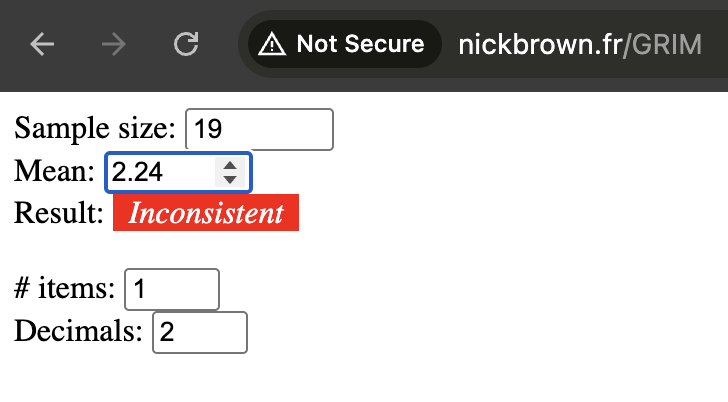
\includegraphics[width=0.5\linewidth]{img/grim/nickbrown's grim test.png}
    \caption{Screenshot of Nick Brown's web app}
\end{figure}
\end{comment}

\subsubsection*{{scrutiny} R package and web app}

The R package \href{https://cran.r-project.org/web/packages/scrutiny/}{scrutiny} implements GRIM and GRIMMER testing (see \href{https://cran.r-project.org/web/packages/scrutiny/vignettes/grim.html}{its vignette on GRIM testing}). GRIM testing can be performed in a single line of code:

\begin{verbatim}
library(scrutiny)
grim(x = "3.51", n = 30, items = 1)
\end{verbatim}

The package also has an \href{https://errors.shinyapps.io/scrutiny}{R Shiny web app} that allows you to run GRIM and GRIMMER with a point-and-click graphical interface. This app has the benefit of allowing you to download a reproducible report of the results.

\begin{comment}
Reese: Again, I doubt this is necessary.
\begin{figure}[h!]
    \centering
    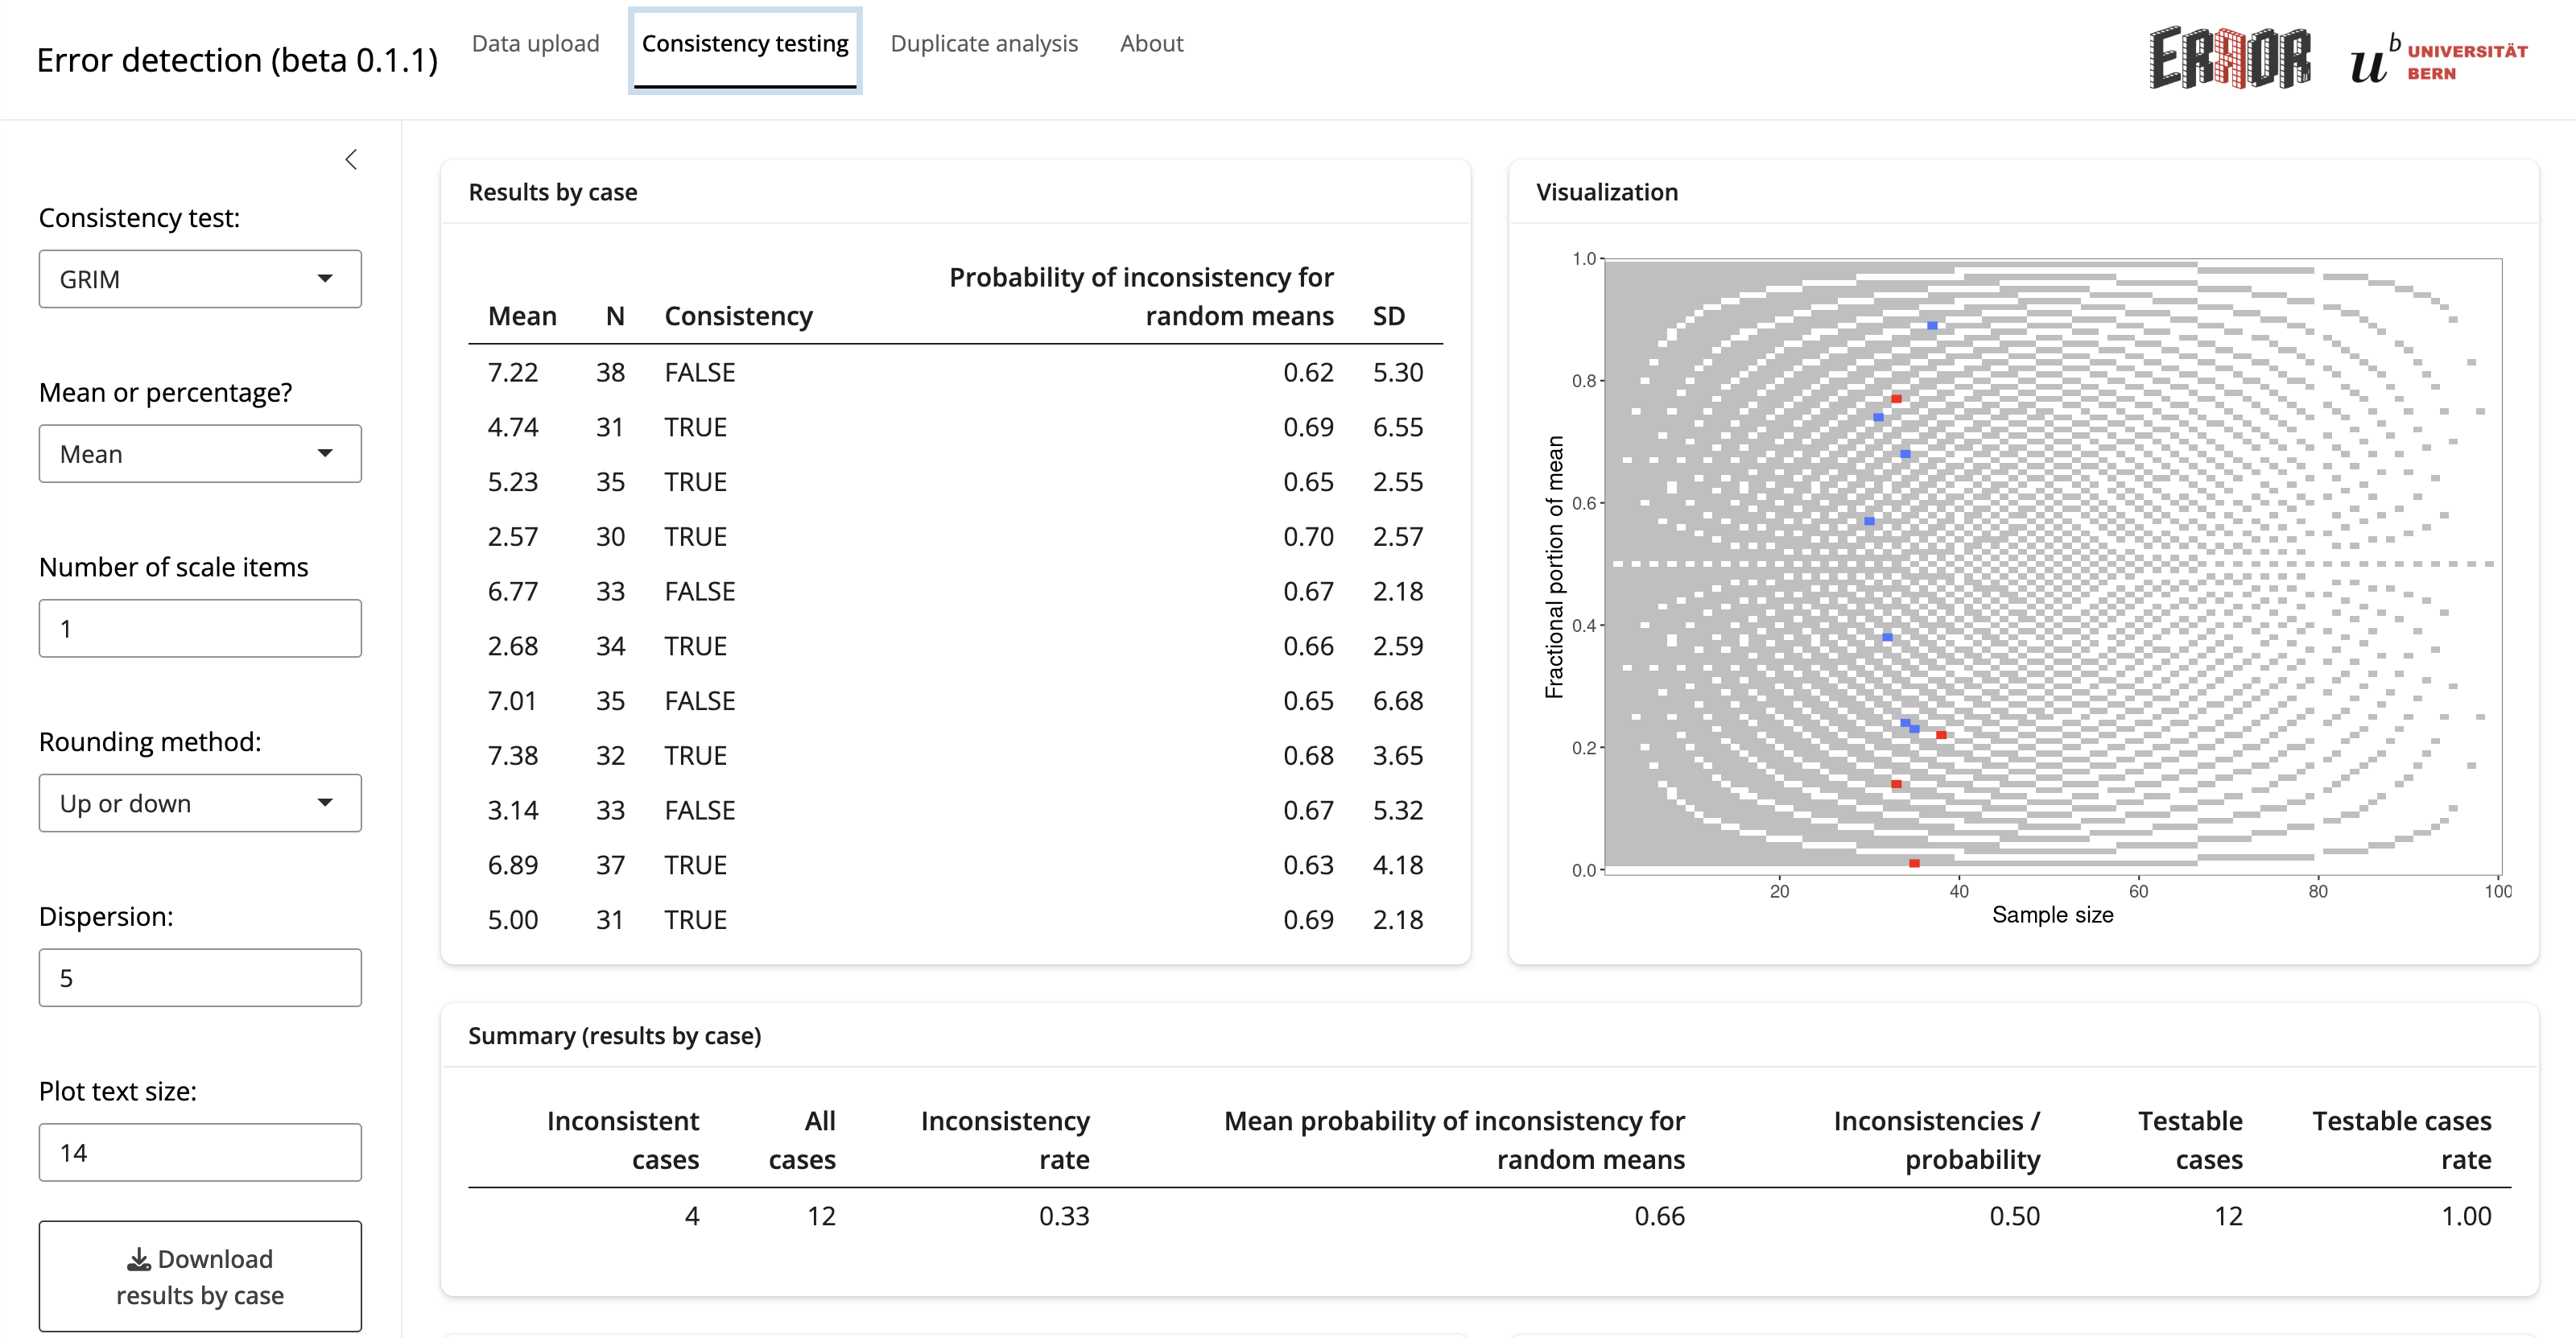
\includegraphics[width=0.5\linewidth]{img/grim/scrutiny web app.png}
    \caption{Screenshot of Lukas Jung's web app}
\end{figure}
\end{comment}

\subsubsection*{rsprite2 R package}

The R package \href{https://cloud.r-project.org/web/packages/rsprite2/index.html}{rsprite2}, an implementation of \href{https://doi.org/10.7287/peerj.preprints.26968v1}{SPRITE (\textit{S}ample \textit{P}arameter \textit{R}econstruction via \textit{I}terative \textit{TE}chniques)}, also contains implementation of GRIM and GRIMMER. See \href{https://lukaswallrich.github.io/rsprite2}{the package's home page}. GRIM can be run in one line of code:
\begin{verbatim}
library(rsprite2)
GRIM_test(mean = 3.51, n_obs = 30, n_items = 1)
\end{verbatim}
Users can optionally produce reports of their results, allowing for reproducible testing.

\begin{comment}
As of this guide's last updated, there are some values of SD that are GRIMMER consistent that \texttt{rscrutiny2::GRIMMER\_test()}currently returns as inconsistent. Therefore, it is recommended to use scrutiny over rsprite2 for GRIM/MER.
\end{comment}

\subsubsection*{{grim} Python package}

The Python package \href{https://pypi.org/project/grim/}{grim} allows for GRIM testing with control over rounding methods.
\begin{verbatim}
from grim import mean_tester
import decimal
print(mean_tester.consistency_check("3.51", "30", 
    decimal.ROUND_HALF_UP))
\end{verbatim}

\subsubsection*{scrutipy Python package}

The package \href{https://pypi.org/project/scrutipy/}{scrutipy} is a Python implementation of the scrutiny R package and has similar functionality.

\subsection*{Example 1: Multiple reported mean values fail GRIM testing}

\href{https://doi.org/10.1177/0269215520923135}{Zemestani and Mozzafari (2020)} report on a clinical trial testing the efficacy of a certain style of therapy on depression. They report a mean age of 23.72 in their intervention group, which has 30 participants. This value is mathematically impossible, even when taking into account different rounding methods and the possibility that the authors averaged only over participants that did not drop out of the study (N = 23). The mean age reported for the control group (25.18 years for N = 30) also fails GRIM testing.

Later in the article, the authors report on their participants mean scores on the \href{https://en.wikipedia.org/wiki/Beck_Depression_Inventory}{Beck Depression Inventory (BDI-II)}, which can take integer values from 0 to 63. All mean BDI-II values for the 29 participants in the control group are mathematically impossible. For instance, the mean BDI-II score at the first timepoint for the control group is reported as 31.92. The closest possible mean scores (rounded to four decimal places here) are 31.8966 (where all scores sum to 925) and 31.9310 (where all scores sum to 926). It is not possible for the sum of all scores to fall between 925 and 926, and hence this mean score fails GRIM testing.

This article was \href{https://doi.org/10.1177/0269215520923135}{retracted in 2025}.

\subsection*{Example 2: Multiple reported mean values fail GRIM testing}

\href{https://doi.org/10.1007/s00520-021-06304-8}{Alizadeh et al. (2021)} report on a clinical trial testing the efficacy of massage therapy on fatigue following chemotherapy. Several reported summary statistics are GRIM-inconsistent. For instance, Table 3 reports the average number of chemotherapy sessions as 5.21 among 44 participants. The closest possible mean values (rounded to four decimal places here) are 5.2045 (a total of 229 chemotherapy sessions) and 5.2272 (a total of 230 chemotherapy sessions). Presumably, it is not possible for a patient to undergo only a fraction of one chemotherapy session (and if it is, the authors did not report how they recorded this).

\subsection*{Additional resources}
\begin{comment}
    

Allard, A. (2018) Analytic-GRIMMER: a new way of testing the possibility of standard deviations. https://aurelienallard.netlify.app/post/anaytic-grimmer-possibility-standard-deviations/

Anaya, J. (2016) The GRIMMER Test: A Method for Testing the Validity of Reported Measures of Variability. https://peerj.com/preprints/2400/

Brown, N., \& Heathers, J. (2017) The GRIM Test: A Simple Technique Detects Numerous Anomalies in the Reporting of Results in Psychology. \textit{Social Psychological and Personality Science.} https://doi.org/10.1177/1948550616673876

Heathers, J. (2016a) The GRIM test: a method for evaluating published research. https://jamesheathers.medium.com/the-grim-test-a-method-for-evaluating-published-research-9a4e5f05e870

Heathers, J. (2016b) The GRIM test: further points, follow-ups, and future directions. https://jamesheathers.medium.com/the-grim-test-further-points-follow-ups-and-future-directions-afd55ff67bb0#.vmgjvdvkf

Heathers, J. (2024) Using GRIM on intermediate figures to retrieve lost descriptive statistics. https://osf.io/m7j2r

Heathers, J. (2025a) An introduction to forensic meta-science. https://jamesheathers.curve.space

Heathers, J. (2025b) Approximately 1 in 7 scientific papers are Ffake. https://osf.io/5rf2m/
  - This article contains follow-up information related to Brown & Heathers (2017) related to potential cases of fraud that were uncovered by that earlier publication.

Hussey, I., Norwood, S. F., Cummins, J., Arslan, R. A., \& Elson, M. (2024). Truncation-Induced Dependency in Summary Statistics: A method for checking the compatibility of reported means, SDs, and Ns given the min and max of the scale. https://github.com/ianhussey/tides
  - Shiny web app: https://errors.shinyapps.io/TIDES/
\end{comment}

\begin{itemize}
    \setlength\itemsep{-0.5em}
    \item \href{https://jamesheathers.medium.com/the-grim-test-a-method-for-evaluating-published-research-9a4e5f05e870}{``The GRIM test: a method for evaluating published research''}

    \item \href{https://jamesheathers.medium.com/the-grim-test-further-points-follow-ups-and-future-directions-afd55ff67bb0\#.vmgjvdvkf}{``The GRIM test: further points, follow-ups, and future directions'' (2016)}

    \item \href{https://doi.org/10.1177/1948550616673876}{``The GRIM Test: A Simple Technique Detects Numerous Anomalies in the Reporting of Results in Psychology'' (2016)}

    \item \href{https://doi.org/10.7287/peerj.preprints.2400v1}{``The GRIMMER Test: A Method for Testing the Validity of Reported Measures of Variability'' (2016)}

    \item \href{https://aurelienallard.netlify.app/post/anaytic-grimmer-possibility-standard-deviations/}{``Analytic-GRIMMER: a new way of testing the possibility of standard deviations'' (2018)}

    \item \href{https://doi.org/10.17605/OSF.IO/M82S6}{``Using GRIM on intermediate figures to retrieve lost descriptive statistics'' (2024)}

    \item \href{https://doi.org/10.5281/zenodo.14871842}{\textit{An Introduction to Forensic Metascience}: ``4.4 GRIM''}

    \item \href{https://github.com/ianhussey/tides}{Truncation-Induced Dependency in Summary Statistics (TIDES): A method for checking the compatibility of reported means, SDs, and Ns given the min and max of the scale}

    \item \href{https://errors.shinyapps.io/TIDES/}{Shiny web app for TIDES}
\end{itemize}
\end{document}